\chapter{Implementação paralelo do PSO}

Executar na Memphis outras funções (esphere, rosenbrock, rastringin)

%----------------------------------------------------------------
\section{Estratégia de paralelismo}
%----------------------------------------------------------------

Texto da seção

%----------------------------------------------------------------
\section{Topologia de comunicação}
%----------------------------------------------------------------

Texto da seção

%----------------------------------------------------------------
\section{Resultados experimentais}
%----------------------------------------------------------------

Nesta seção apresentaremos os resultados das execuções do algoritmo PSO na plataforma Memphis.
A coluna “Nº de elementos processadores” se refere à quantidade do mestre somado aos processadores escravos, exceto ao que se refere com 1 que é o algoritmo serial. Já a coluna “Tempo algoritmo (ticks)” se refere ao tempo de execução do algoritmo somente com o tempo em ticks, cada tick equivale a 10µs. A coluna “Tempo plataforma (ticks)” se refere ao tempo do algoritmo somado ao tempo da preparação da plataforma. A coluna “Speedup”
Nas tabelas abaixo estão os valores de cada execução do algoritmo na plataforma Memphis variando a população e as interações:

\begin{table}[h]{12cm}
    \caption{Cenário de teste com população igual a 100 e 20 iterações}
    \label{tbl:taylor-vortex-parameters}
    \begin{tabular}{llll}
        \hline
        \shortstack[l]{Nº de elementos \\ processadores} & \shortstack[l]{Tempo algoritmo \\ (ticks)} & \shortstack[l]{Tempo plataforma \\ (ticks)} & Speedup \\
        \hline
        1 & 1.615.530 & 1.617.079 & 1,00 \\
        2 & 1.950.193 & 1.951.735 & 0,83 \\
        3 & 1.024.344 & 1.025.892 &	1,58 \\
        4 & 720.708   & 722.186   & 2,24 \\
        5 & 589.084   & 590.562   & 2,74 \\
        6 & 503.492   & 504.970   & 3,21 \\
        \hline
    \end{tabular}
    %\legend{Texto da legenda. (Opcional)}
    %\source{Citação da fonte ou `O autor'. (opcional)}
\end{table}

\begin{table}[h]{12cm}
    \caption{Cenário de teste com população igual a 200 e 20 iterações}
    \label{tbl:taylor-vortex-parameters}
    \begin{tabular}{llll}
        \hline
        \shortstack[l]{Nº de elementos \\ processadores} & \shortstack[l]{Tempo algoritmo \\ (ticks)} & \shortstack[l]{Tempo plataforma \\ (ticks)} & Speedup \\
        \hline
        1 & 3.175.949 & 3.177.498 & 1,00 \\
        2 & 3.802.205 & 3.803.747 & 0,84 \\
        3 & 1.951.996 & 1.953.544 &	1,63 \\
        4 & 1.350.049 & 1.351.597 & 2,35 \\
        5 & 1.048.768 & 1.050.316 & 3,03 \\
        6 & 876.873   & 878.351   & 3,62 \\
        \hline
    \end{tabular}
    %\legend{Texto da legenda. (Opcional)}
    %\source{Citação da fonte ou `O autor'. (opcional)}
\end{table}

\begin{table}[h]{12cm}
    \caption{Cenário de teste com população igual a 300 e 20 iterações}
    \label{tbl:taylor-vortex-parameters}
    \begin{tabular}{llll}
        \hline
        \shortstack[l]{Nº de elementos \\ processadores} & \shortstack[l]{Tempo algoritmo \\ (ticks)} & \shortstack[l]{Tempo plataforma \\ (ticks)} & Speedup \\
        \hline
        1 & 4.732.875 & 4.734.424 & 1,00 \\
        2 & 5.657.594 & 5.659.136 & 0,84 \\
        3 & 2.875.817 & 2.877.365 &	1,65 \\
        4 & 1.960.693 & 1.962.241 & 2,41 \\
        5 & 1.511.697 & 1.513.245 & 3,13 \\
        6 & 1.245.103 & 1.246.651 & 3,80 \\
        \hline
    \end{tabular}
    %\legend{Texto da legenda. (Opcional)}
    %\source{Citação da fonte ou `O autor'. (opcional)}
\end{table}

\begin{table}[h]{12cm}
    \caption{Cenário de teste com população igual a 400 e 20 iterações}
    \label{tbl:taylor-vortex-parameters}
    \begin{tabular}{llll}
        \hline
        \shortstack[l]{Nº de elementos \\ processadores} & \shortstack[l]{Tempo algoritmo \\ (ticks)} & \shortstack[l]{Tempo plataforma \\ (ticks)} & Speedup \\
        \hline
        1 & 6.281.550 & 6.283.099 & 1,00 \\
        2 & 7.515.159 & 7.516.701 & 0,84 \\
        3 & 3.805.477 & 3.807.025 &	1,65 \\
        4 & 2.574.297 & 2.575.845 & 2,44 \\
        5 & 1.976.616 & 1.978.164 & 3,18 \\
        6 & 1.613.632 & 1.615.180 & 3,89 \\
        \hline
    \end{tabular}
    %\legend{Texto da legenda. (Opcional)}
    %\source{Citação da fonte ou `O autor'. (opcional)}
\end{table}

\begin{table}[h]{12cm}
    \caption{Cenário de teste com população igual a 500 e 20 iterações}
    \label{tbl:taylor-vortex-parameters}
    \begin{tabular}{llll}
        \hline
        \shortstack[l]{Nº de elementos \\ processadores} & \shortstack[l]{Tempo algoritmo \\ (ticks)} & \shortstack[l]{Tempo plataforma \\ (ticks)} & Speedup \\
        \hline
        1 & 7.844.240 & 7.845.789 & 1,00 \\
        2 & 9.373.217 & 9.374.760 & 0,84 \\
        3 & 4.736.120 & 4.737.668 &	1,66 \\
        4 & 3.202.018 & 3.203.566 & 2,45 \\
        5 & 2.440.490 & 2.442.038 & 3,21 \\
        6 & 1.984.755 & 1.986.303 & 3,95 \\
        \hline
    \end{tabular}
    %\legend{Texto da legenda. (Opcional)}
    %\source{Citação da fonte ou `O autor'. (opcional)}
\end{table}

\begin{graph}[h]{16cm}
    \caption{Cenário de teste com 20 iterações}
        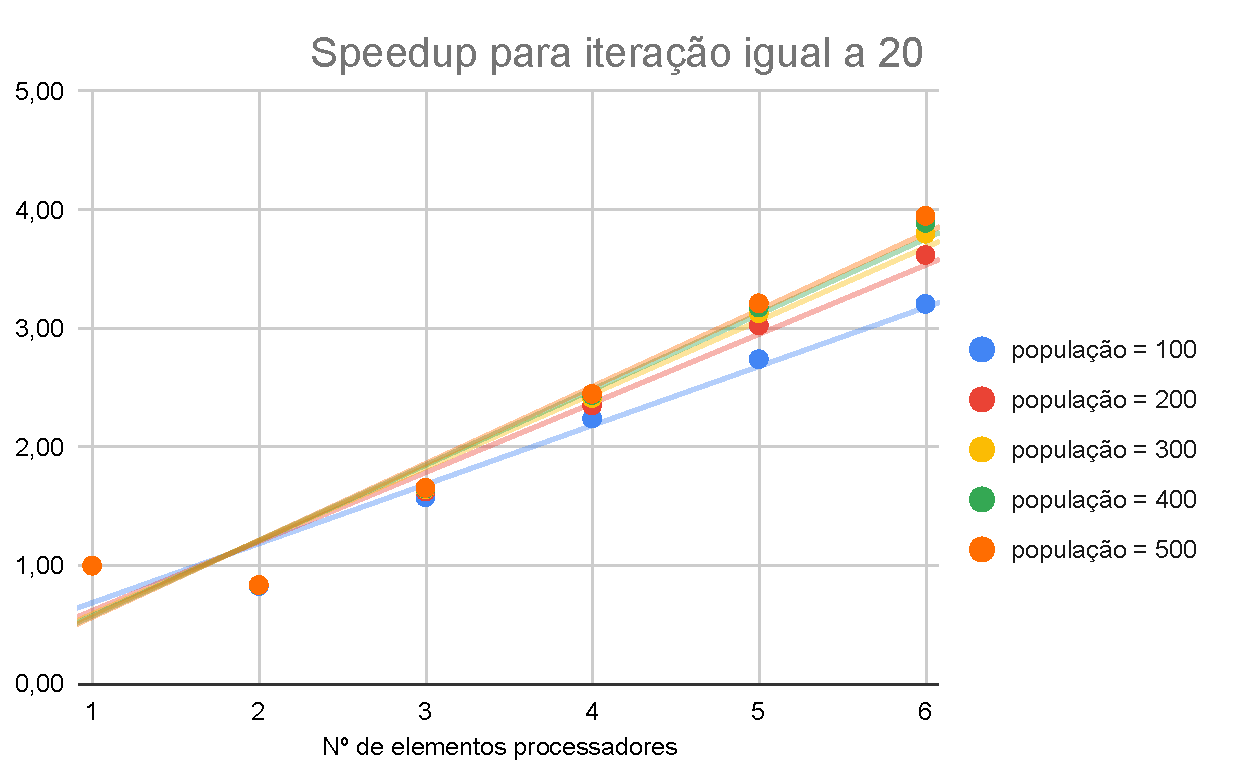
\includegraphics[width=14cm]{graficos/Speedup para iteração igual a 20.pdf}
\end{graph}

\begin{graph}[h]{16cm}
    \caption{Cenário de teste com 30 iterações}
        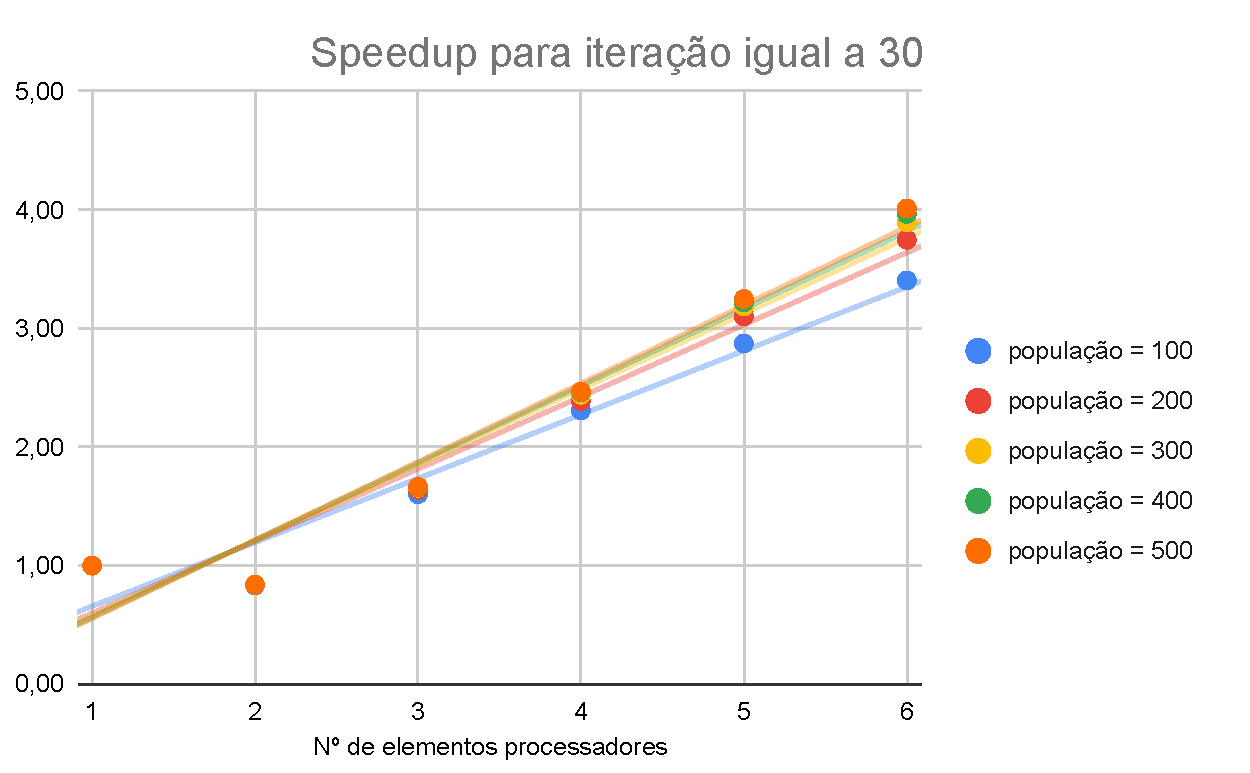
\includegraphics[width=14cm]{graficos/Speedup para iteração igual a 30.pdf}
\end{graph}

\begin{graph}[h]{16cm}
    \caption{Cenário de teste com 40 iterações}
        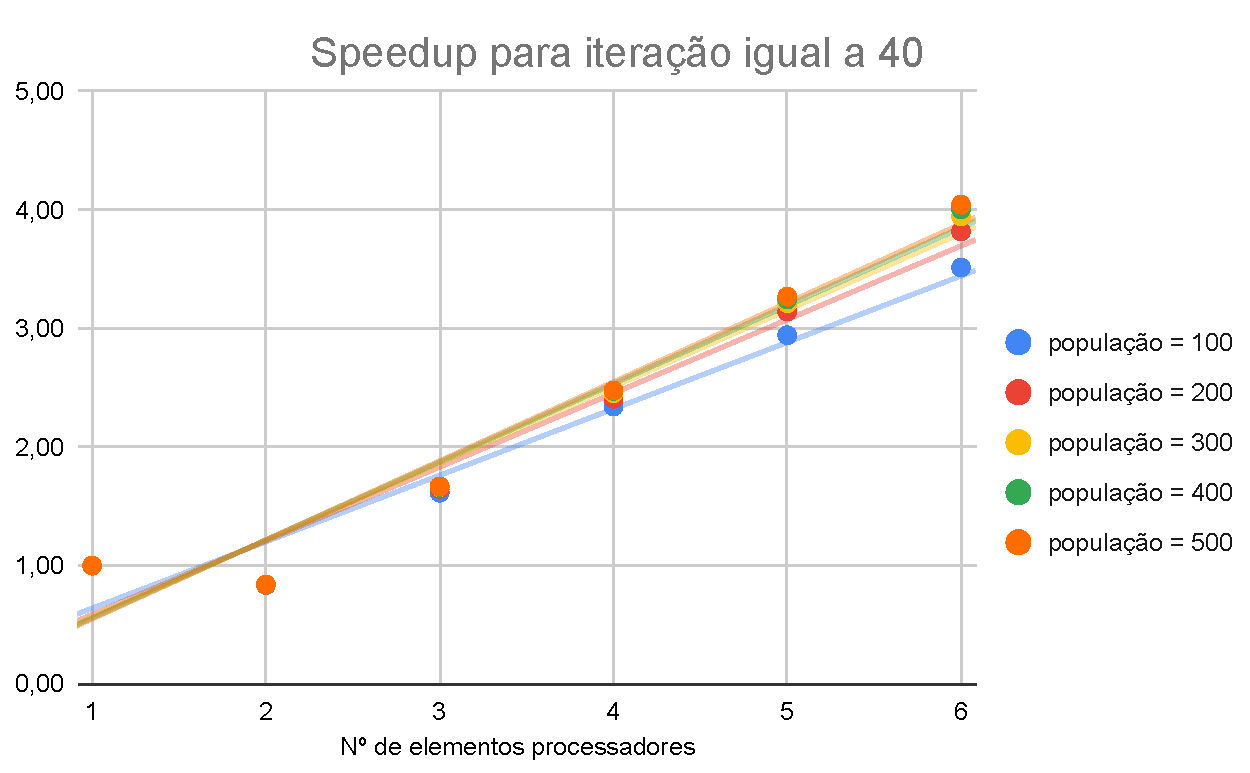
\includegraphics[width=14cm]{graficos/Speedup para iteração igual a 40.pdf}
\end{graph}

\begin{graph}[h]{16cm}
    \caption{Cenário de teste com 50 iterações}
    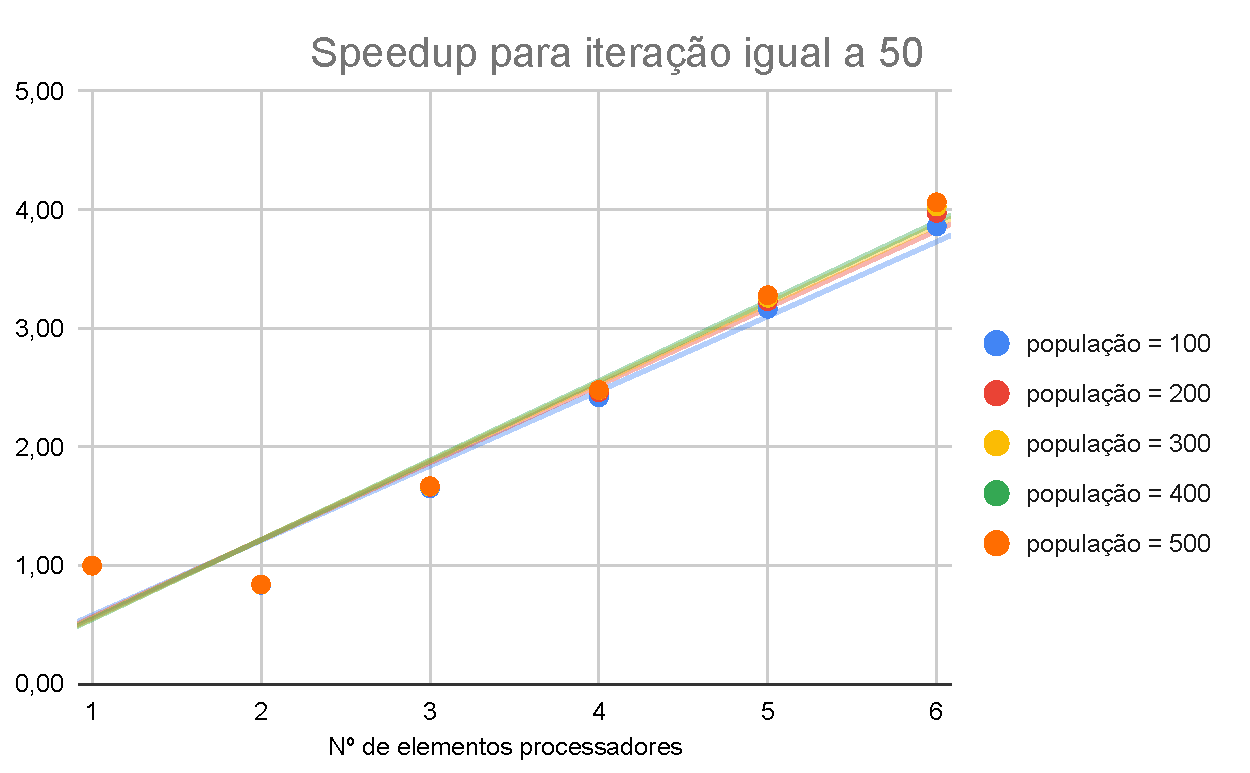
\includegraphics[width=14cm]{graficos/Speedup para iteração igual a 50.pdf}
\end{graph}

%\begin{figure}[ht]{12cm}
%  \begin{center}
%    \leavevmode
%    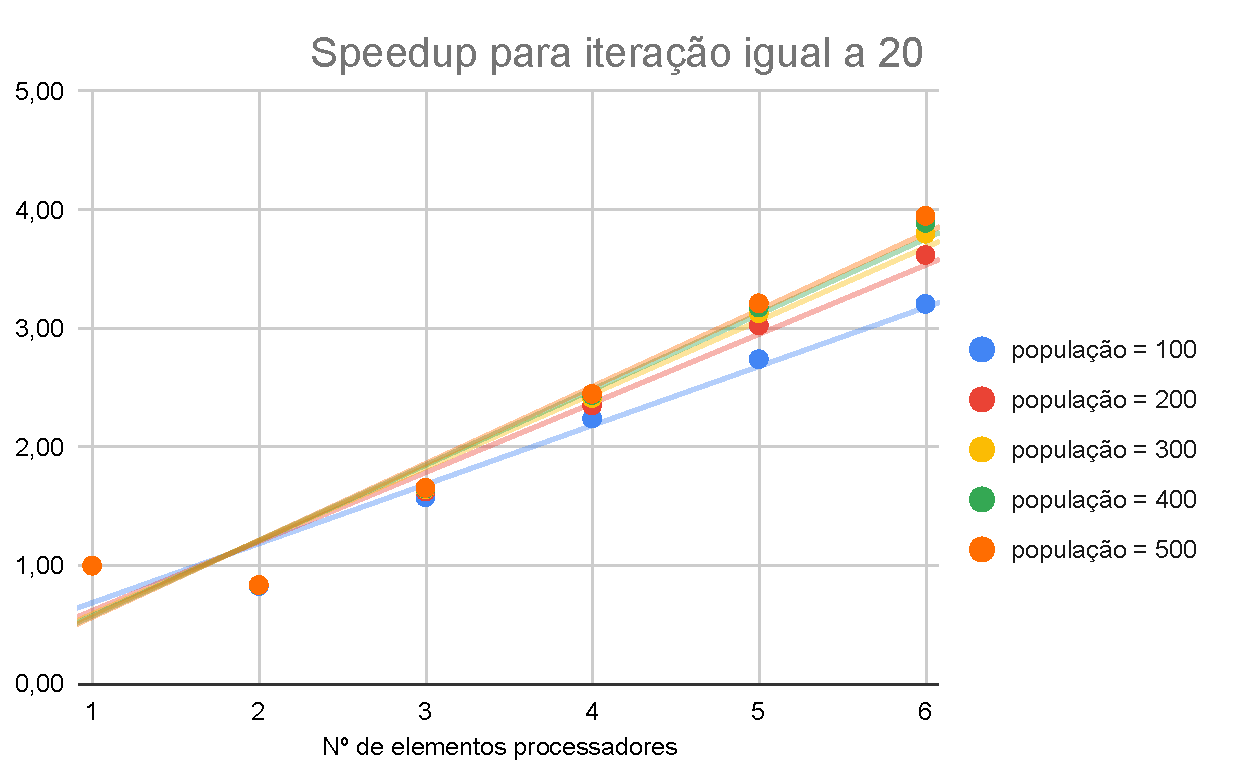
\includegraphics[width=0.65\textwidth]{graficos/Speedup para iteração igual a 20.pdf}
%    \caption{Two element linear array (from \cite{gross15})}
%    \label{fig:2elem}
%  \end{center}
%\end{figure}

Lei de Amdahl

\begin{align}
    &G=\frac{1}{S+\frac{1-S}{n}}
\end{align}